\chapter{Oxygen Transport Results and Discussion}
\label{ch:o2results}

\begin{keybox}[Status of the results in this chapter]
All results here are \textbf{model predictions} \tagM\ from the closed forms of \cref{ch:o2analytical} and the 1.5-D model. They use the validated lubrication flow, but the uptake parameters are illustrative (\cref{tab:o2params}). No oxygen CFD or measurement was available. The ``analytical against numerical'' comparison is between the closed forms and the numerically integrated reduced-order model, not against Fluent.
\end{keybox}

\section{Axial distribution of oxygen at the cell layer}

\Cref{fig:o2_axial} shows the oxygen concentration on the floor along the axis for the three flow rates and the three lid conditions. \Cref{tab:o2_results} gives the station values and summary metrics. The imaging window is $5\le x\le\SI{40}{mm}$.

\begin{figure}[htbp]
\centering
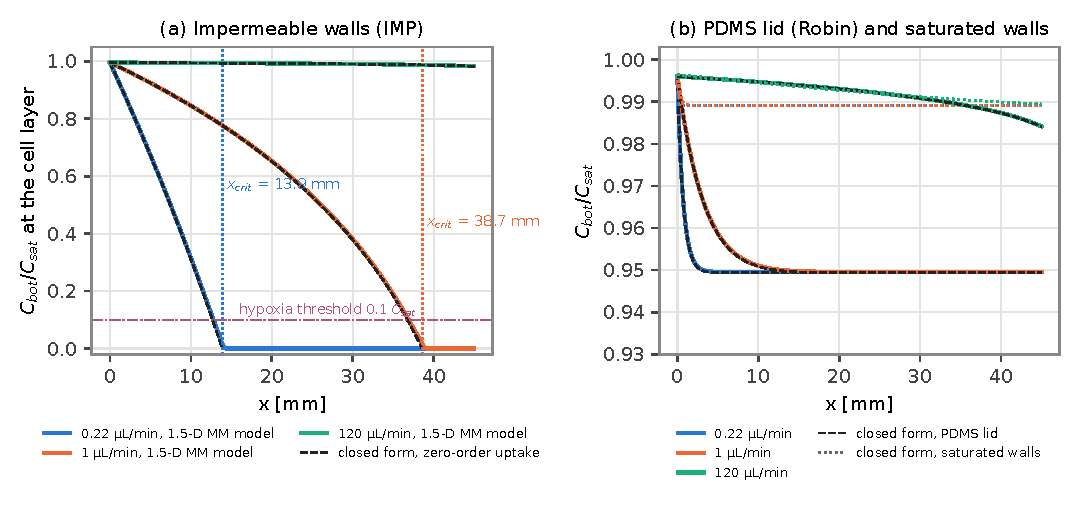
\includegraphics[width=\linewidth]{oxygen_axial_profiles.pdf}
\caption{Oxygen at the cell layer along the channel, $\Cbot/\Csat$ \tagM. Coloured lines: 1.5-D model with Michaelis--Menten uptake. Black dashed lines: closed forms with zero-order uptake, \cref{eq:ox_imp_bot} and \cref{eq:ox_pdms}. Dotted lines in (b): closed form for a saturated lid. (a) With impermeable walls the floor becomes anoxic beyond $x_{\mathrm{crit}}=13.9$ and \SI{38.7}{mm} at 0.22 and \SI{1}{\uLmin}. (b) With a \SI{5}{mm} PDMS lid the concentration relaxes within 1--\SI{3}{mm} to the lid equilibrium $0.949\,\Csat$, independent of $Q$. At \SI{120}{\uLmin} convection dominates and all three walls give 0.98--\SI{1.00}{}$\,\Csat$.}
\label{fig:o2_axial}
\end{figure}

\begin{table}[htbp]
\centering
\caption{Oxygen at the cell layer, $\Cbot/\Csat$, from the 1.5-D model with baseline parameters \tagM. Window = $5\le x\le\SI{40}{mm}$; ``hypoxic'' = area fraction of the window with $\Cbot<0.1\,\Csat$.}
\label{tab:o2_results}
\small
\resizebox{\linewidth}{!}{%
\begin{tabular}{@{}llccccccccc@{}}
\toprule
$Q$ & Lid & S1 & S2 & S3 & S4 & S5 & Mean in & Min in & Hypoxic & $\Cb_{\mathrm{out}}/\Csat$\\
{[}\ulmin{]} & & & & & & & window & window & fraction & ($x=\SI{45}{mm}$)\\
\midrule
0.22 & IMP  & 0.675 & 0.000 & 0.000 & 0.000 & 0.000 & 0.050 & 0.000 & 0.87 & 0.000\\
0.22 & PDMS & 0.950 & 0.950 & 0.950 & 0.950 & 0.950 & 0.950 & 0.950 & 0 & 0.955\\
0.22 & SAT  & 0.989 & 0.989 & 0.989 & 0.989 & 0.989 & 0.989 & 0.989 & 0 & 0.995\\
\addlinespace
1 & IMP  & 0.925 & 0.757 & 0.531 & 0.190 & 0.000 & 0.426 & 0.000 & 0.18 & 0.000\\
1 & PDMS & 0.959 & 0.950 & 0.950 & 0.950 & 0.950 & 0.950 & 0.950 & 0 & 0.955\\
1 & SAT  & 0.989 & 0.989 & 0.989 & 0.989 & 0.989 & 0.989 & 0.989 & 0 & 0.995\\
\addlinespace
120 & IMP  & 0.995 & 0.994 & 0.992 & 0.989 & 0.983 & 0.991 & 0.987 & 0 & 0.987\\
120 & PDMS & 0.995 & 0.994 & 0.992 & 0.989 & 0.984 & 0.991 & 0.987 & 0 & 0.988\\
120 & SAT  & 0.995 & 0.994 & 0.992 & 0.991 & 0.989 & 0.992 & 0.990 & 0 & 0.995\\
\bottomrule
\end{tabular}}
\end{table}

\section{Discussion of the guiding questions}

\paragraph{1. How does the oxygen concentration vary in space?} Along the channel, the concentration is governed by \cref{eq:ox_cupA}: it falls in proportion to the cell area already passed, unless the lid replaces what is consumed. Across the gap it varies by at most \SI{1.1}{\percent} (\cref{fig:o2_z}), because diffusion across \SI{145}{\micro\metre} takes \SI{7}{s} while the medium spends 17--\SI{76}{min} in the culture section at the two culture flow rates. Across the width, the reduced-order model assumes no variation. The CFD flow field, however, shows a \SI{0.13}{mm} side-wall layer of slower fluid (\cref{sec:val_transverse}), where the residence time is longer and the depletion with impermeable walls will be stronger.

\paragraph{2. Where are the highest and lowest concentrations?} The highest concentrations are at the inlet, $\Csat$ by definition. With impermeable walls the lowest are downstream: the floor is anoxic beyond \SI{13.9}{mm} at \SI{0.22}{\uLmin} (\SI{87}{\percent} of the imaging window hypoxic) and beyond \SI{38.7}{mm} at \SI{1}{\uLmin} (\SI{18}{\percent} hypoxic, in the S4--S5 region). With a PDMS lid, the minimum, $0.949\,\Csat$, is reached a few millimetres from the inlet and then stays constant.

\paragraph{3. Relative importance of convection and diffusion.} Diffusion controls transport across the gap and convection controls transport along the channel ($\Pe_L\ge421$, $t_D/t_{\mathrm{res}}\le\num{7e-3}$ at the culture flow rates). The competition that matters is between convective \emph{supply} and \emph{uptake}, measured by $\Da_{\mathrm{conv}}$: 7.06, 1.55 and 0.013. The ``P\'eclet number'' in the usual sense does not decide oxygen availability here. $\Pe_h$ is 1.2 at \SI{0.22}{\uLmin}, and yet the floor is anoxic over most of the channel.

\paragraph{4. How does the velocity field influence oxygen transport?} Only through the flow rate (the convective capacity $Q\Csat$) and the shape of the profile across the gap (the factors 13/35 and 9/70 in \cref{eq:ox_superpos}). Because the flow is a Stokes flow, the oxygen field at a given $Q$ is independent of the absolute velocity magnitude. The \SI{-5}{\percent} CFD offset therefore has no bearing on these results.

\paragraph{5. Does the geometry help or hinder oxygen delivery?} It hinders it in the low-shear region. In a straight channel of width $w_1$, the cell area upstream of $x=\SI{40}{mm}$ would be \SI{40}{mm^2}; in the hyperbolic channel it is \SI{80.5}{mm^2}. Per unit flow, the downstream cells receive medium that has fed twice as many cells. The geometry that creates a linear shear gradient also creates a steepening oxygen gradient in the same direction (\cref{eq:ox_imp_bot}).

\paragraph{6. How does oxygen change along the flow direction?} With impermeable walls, it falls in proportion to $\ln[L/(L-x)]$, slowly at first and then faster, until anoxia at $x_{\mathrm{crit}}$. Beyond that point there is a sharp transition (decay length about \SI{0.1}{mm}, \cref{sec:ox_mm}). With a PDMS lid, the concentration falls exponentially in $A(x)$ to a plateau. At \SI{120}{\uLmin} it falls almost linearly by 1--\SI{2}{\percent}.

\paragraph{7. Role of the wall boundary condition.} The lid condition is decisive at the culture flow rates (\cref{fig:o2_axial}). With an impermeable lid, oxygen availability is set by the flow and is poor. With a \SI{5}{mm} PDMS lid it is set by the lid and is good at every flow rate, because the lid can supply 25 times the maximum uptake ($\Phi_{\mathrm{PDMS}}=25.1$). With a PDMS lid at 0.22 and \SI{1}{\uLmin}, about \SIrange{97}{99}{\percent} of the oxygen consumed is supplied through the lid and only 1--\SI{3}{\percent} by the flow. At \SI{120}{\uLmin} the lid supplies only about \SI{11}{\percent}. Whether cells in this device are hypoxic is therefore decided by the PDMS, not by the flow, provided the lid is exposed to incubator air and has its nominal permeability.

\paragraph{8. Influence of the consumption model.} With Michaelis--Menten kinetics and $\Csat/\Km=283$, the uptake is effectively zero order wherever $\Cbot>0.03\,\Csat$. The closed forms with zero-order uptake coincide with the numerical model up to $x_{\mathrm{crit}}$ (\cref{fig:o2_axial}a), and the choice of $\Km$ only affects the sub-millimetre transition zone. A first-order model, $q=(\qmax/\Km)C$, would be wrong by a factor of up to 280 at normoxic concentrations. The parameters that control the results are $\qmax$ (cell density $\times$ uptake per cell) and $\kp$, not $\Km$.

\paragraph{9. Effect of the flow rate.} With impermeable walls, increasing $Q$ moves $x_{\mathrm{crit}}$ downstream, in proportion to $1-\exp(-Q\Csat/\qmax w_1L)$, and removes anoxia altogether above $Q_{\min}=\SI{1.55}{\uLmin}$. At \SI{120}{\uLmin} the depletion is \SI{1.3}{\percent}. With a PDMS lid the flow rate barely matters at 0.22 and \SI{1}{\uLmin} (equilibrium $0.949\,\Csat$), and at \SI{120}{\uLmin} convection keeps the concentration even higher (0.983--$0.995\,\Csat$).

\section{Shear and oxygen together}

\Cref{fig:o2_tau} plots the oxygen at the cell layer against the local wall shear over the imaging window. With impermeable walls, the cells exposed to the lowest shear are also the cells starved of oxygen. At \SI{0.22}{\uLmin} every cell below about \SI{0.008}{\dyncm} is anoxic, and at \SI{1}{\uLmin} every cell below about \SI{0.010}{\dyncm}. A shear-response experiment in an impermeable device would therefore confound shear and hypoxia in exactly the part of the shear range that the device was designed to explore. With a PDMS lid the oxygen is uniform ($0.95\,\Csat$) across the whole shear range, so shear is the only variable.

\begin{figure}[htbp]
\centering
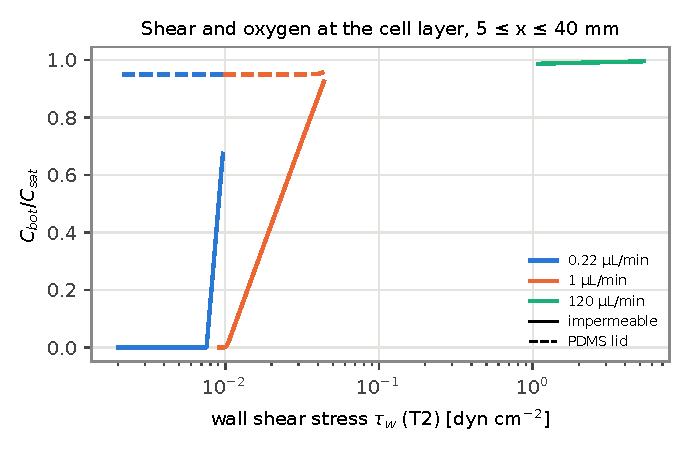
\includegraphics[width=0.62\linewidth]{oxygen_vs_shear.pdf}
\caption{Oxygen at the cell layer against wall shear (T2) for $5\le x\le\SI{40}{mm}$ \tagM. Solid: impermeable walls. Dashed: \SI{5}{mm} PDMS lid. With impermeable walls the lowest shear coincides with anoxia at 0.22 and \SI{1}{\uLmin}.}
\label{fig:o2_tau}
\end{figure}

\section{Quantitative interpretation}

\begin{table}[htbp]
\centering
\caption{Oxygen budget of the culture section \tagM. Rates in \si{mol/s}; ``demand met'' is the actual uptake divided by the maximum uptake $\qmax A_{\mathrm{cells}}$.}
\label{tab:o2_budget}
\small
\begin{tabular}{@{}lccc@{}}
\toprule
Quantity & \SI{0.22}{\uLmin} & \SI{1}{\uLmin} & \SI{120}{\uLmin}\\
\midrule
Convective supply $Q\Csat$ & \num{6.53e-13} & \num{2.97e-12} & \num{3.56e-10}\\
Maximum uptake $\qmax A_{\mathrm{cells}}$ & \num{4.61e-12} & \num{4.61e-12} & \num{4.61e-12}\\
Maximum lid supply $\kp\Csat A_{\mathrm{cells}}$ & \num{1.16e-10} & \num{1.16e-10} & \num{1.16e-10}\\
Actual uptake, IMP & \num{6.53e-13} & \num{2.97e-12} & \num{4.59e-12}\\
Demand met, IMP & \SI{14}{\percent} & \SI{64}{\percent} & \SI{99.6}{\percent}\\
Actual uptake, PDMS & \num{4.59e-12} & \num{4.59e-12} & \num{4.59e-12}\\
Depletion at $x=\SI{45}{mm}$, IMP ($1-\Cb/\Csat$) & \SI{100}{\percent} & \SI{100}{\percent} & \SI{1.3}{\percent}\\
Depletion at $x=\SI{45}{mm}$, PDMS & \SI{4.5}{\percent} & \SI{4.5}{\percent} & \SI{1.2}{\percent}\\
Diffusion time across gap $t_D$ [s] & 7.0 & 7.0 & 7.0\\
Residence time $t_{\mathrm{res}}$ [s] & 4553 & 1002 & 8.3\\
Onset of anoxia, IMP [mm] & 13.9 & 38.7 & none\\
PDMS relaxation length $x^*$ [mm] & 0.71 & 3.1 & $>45$\\
\bottomrule
\end{tabular}
\end{table}

\Cref{tab:o2_budget} gives the budget. With impermeable walls at \SI{0.22}{\uLmin} the flow delivers only \SI{14}{\percent} of what the cells could consume, and at \SI{1}{\uLmin} \SI{64}{\percent}. In both cases the outlet medium is fully depleted. The flux of oxygen into the cell layer is $\qmax=\SI{4e-8}{mol.m^{-2}.s^{-1}}$ wherever $\Cbot\gg\Km$ and falls to zero in the anoxic zone. With a PDMS lid the full demand is met at every flow rate.

\paragraph{Sensitivity.} \Cref{tab:o2_sens} and \cref{fig:o2_design} show how the conclusions depend on the uncertain parameters. Using the closed forms, the effects can be read off directly:
\begin{itemize}
\item $\qmax$ dominates. The plausible range of \num{0.5e-8} to \SI{50e-8}{mol.m^{-2}.s^{-1}} changes $Q_{\min}$ from 0.19 to \SI{19}{\uLmin}.
\item With a PDMS lid the floor stays above $0.87\,\Csat$ up to $\qmax=\SI{1e-7}{mol.m^{-2}.s^{-1}}$. Only at the extreme value of \num{5e-7} would it fall to $0.37\,\Csat$.
\item $\Csat$, $D$ and the lid properties change the results by a few percent.
\end{itemize}
The two quantities that must be measured before any oxygen conclusion is drawn for Caco-2 or A549 cells are therefore the oxygen consumption per cell and the cell density at confluence.

\begin{table}[htbp]
\centering
\caption{Sensitivity of the closed-form predictions \tagM. Bold = baseline. $C_{\mathrm{bot},\infty}$ is the PDMS-lid equilibrium, \cref{eq:ox_pdms_inf}.}
\label{tab:o2_sens}
\small
\resizebox{\linewidth}{!}{%
\begin{tabular}{@{}lccccc@{}}
\toprule
Case & $Q_{\min}$ [\ulmin] & $x_{\mathrm{crit}}$ at 0.22 [mm] & $x_{\mathrm{crit}}$ at 1 [mm] & $\Phi_{\mathrm{PDMS}}$ & $C_{\mathrm{bot},\infty}/\Csat$ (PDMS)\\
\midrule
\textbf{Baseline} & \textbf{1.55} & \textbf{13.9} & \textbf{38.7} & \textbf{25.1} & \textbf{0.949}\\
$\qmax=\num{0.5e-8}$ & 0.19 & none & none & 201 & 0.994\\
$\qmax=\num{10e-8}$ & 3.88 & 6.1 & 22.4 & 10.1 & 0.873\\
$\qmax=\num{50e-8}$ & 19.4 & 1.3 & 5.6 & 2.0 & 0.367\\
$\Csat=0.167$ / 0.200 & 1.65 / 1.38 & 13.2 / 15.3 & 37.6 / 40.6 & 23.6 / 28.2 & 0.946 / 0.955\\
$D=\SI{2.6e-9}{m^2/s}$ & 1.55 & 13.9 & 38.7 & 25.1 & 0.948\\
PDMS 600 Barrer & 1.55 & 13.9 & 38.7 & 18.9 & 0.936\\
PDMS 8 mm / 3 mm thick & 1.55 & 13.9 & 38.7 & 15.7 / 41.9 & 0.926 / 0.965\\
\bottomrule
\end{tabular}}
\end{table}

\begin{figure}[htbp]
\centering
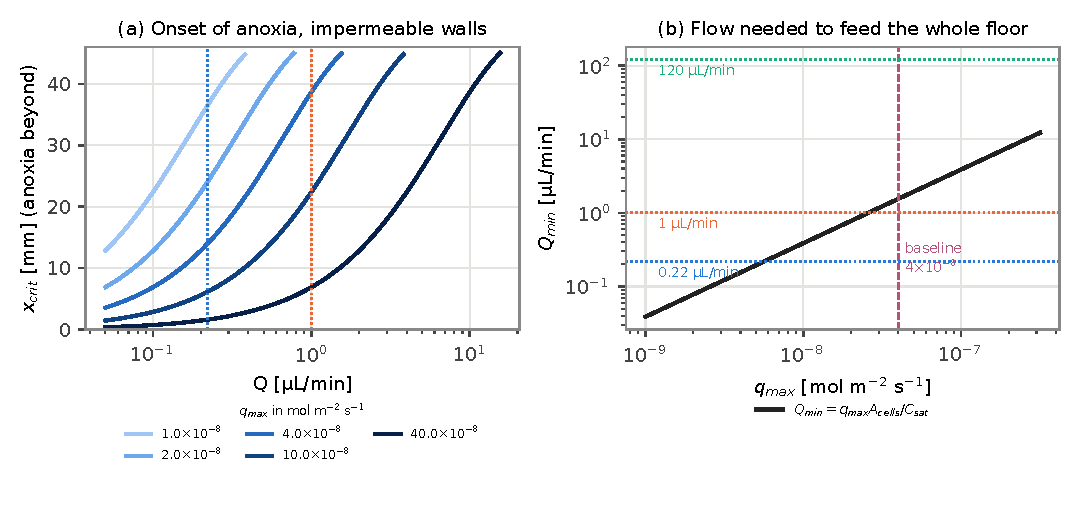
\includegraphics[width=\linewidth]{oxygen_design_map.pdf}
\caption{Design maps from the closed forms (impermeable walls) \tagM. (a) Position beyond which the floor is anoxic, \cref{eq:ox_xcrit}, against flow rate for a range of $\qmax$. Dotted lines: 0.22 and \SI{1}{\uLmin}. (b) Minimum flow rate that feeds the whole culture section by convection alone, \cref{eq:ox_qmin}.}
\label{fig:o2_design}
\end{figure}

\section{Engineering implications}

\begin{enumerate}
\item \textbf{Low shear and low oxygen coincide in this geometry.} The device delivers its lowest shear exactly where its oxygen supply by convection is lowest. In a device with impermeable walls (glass, thermoplastics, or PDMS whose surface is sealed or coated) a shear experiment at \SI{\le1}{\uLmin} would expose the downstream cells to hypoxia. This would be invisible in a flow simulation.
\item \textbf{A PDMS lid keeps the cells oxygenated in the model.} With a \SI{5}{mm} PDMS lid exposed to incubator air, the model predicts $\Cbot\ge0.95\,\Csat$ everywhere, at any flow rate. The device as published is therefore probably well oxygenated, but this depends on the lid being permeable in practice. Measurements in perfused PDMS reactors have shown axial oxygen gradients despite PDMS walls \citep{Mehta2007}. Immersing the device in water, as suggested in the protocol to limit bubbles \citep{Delon2020}, would add a transport resistance. These effects should be quantified (with oxygen-sensing films or probes) before the device is used for long-term studies at low flow.
\item \textbf{Operational levers.} With an impermeable device, run at $Q>Q_{\min}=\qmax A_{\mathrm{cells}}/\Csat$. With the baseline uptake this is \SI{1.55}{\uLmin}, which raises the shear accordingly. Alternatively, oxygenate the medium above air saturation (raising $\Csat$), or seed at lower density (lowering $\qmax$).
\item \textbf{Geometric levers.} The shear scales as $\taw\propto Q/(h^2w)$ and the oxygen supply as $Q$. To reach a target shear with more oxygen, increase the height: at constant shear $Q\propto h^2$. Doubling $h$ from 145 to \SI{290}{\micro\metre} would allow four times the flow at the same shear and would cut $\Da_{\mathrm{conv}}$ by four. The cost is thicker side-wall layers ($\delta\propto h$) and a weaker Hele-Shaw approximation ($h/w$ doubles). Reducing $w_{\max}/w_1$ or $L$ reduces the cell area, and hence the uptake, but also the shear range. A thinner PDMS lid increases $\Phi_{\mathrm{PDMS}}$ in proportion to $1/t_{\mathrm{PDMS}}$.
\end{enumerate}

\begin{keybox}[Answer to RQ4--RQ5]
The widening geometry accumulates cell area faster than length, so the cells in the low-shear, downstream region receive the most depleted medium. With impermeable walls and illustrative uptake, convection cannot feed the cells below $Q_{\min}=\SI{1.55}{\uLmin}$: anoxia is predicted beyond \SI{13.9}{mm} (\SI{0.22}{\uLmin}) and \SI{38.7}{mm} (\SI{1}{\uLmin}), coinciding with the lowest shear. A \SI{5}{mm} PDMS lid can supply 25 times the uptake and would hold the cell layer at $0.95\,\Csat$ at every flow rate. Oxygen availability in this device is therefore decided by the walls and the cell uptake, not by the flow. The key unknowns are the measured uptake rate and the effective permeability of the lid.
\end{keybox}
